\documentclass[a4paper,12pt]{report}

% ------------------------
% Pacchetti di base
% ------------------------
\usepackage[utf8]{inputenc}
\usepackage[T1]{fontenc}
\usepackage[italian]{babel}
\usepackage{graphicx}
\usepackage{geometry}
\geometry{margin=3cm}
\usepackage{setspace}
\onehalfspacing % interlinea 1.5

% ------------------------
% Inizio documento
% ------------------------
\begin{document}

% ------------------------
% Frontespizio
% ------------------------
\begin{titlepage}
    \centering
    
    % Logo in alto
    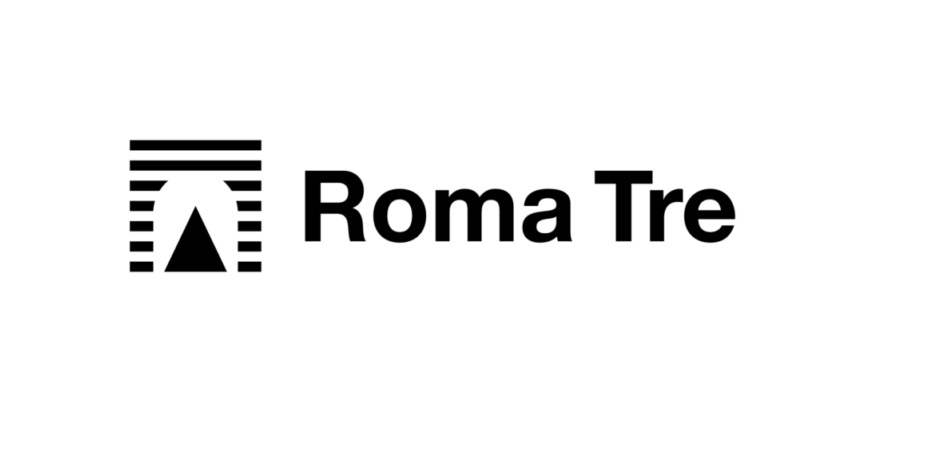
\includegraphics[width=6cm]{tesi/logo_uniroma3.jpeg}\par\vspace{0.5cm}
    
    {\large UNIVERSITÀ DEGLI STUDI ROMA TRE}\par
    \vspace{0.2cm}
    {\normalsize Dipartimento di Ingegneria Civile, Informatica e delle Tecnologie Aeronautiche}\par
    {\normalsize Corso di Laurea Triennale in Ingegneria Informatica}\par
    \vspace{1.5cm}
    
    {\large \textbf{Tesi di Laurea Triennale}}\par
    \vspace{1.5cm}
    
    {\Large \textbf{Sfruttare la fragility di un timetable \\ 
    per l'inserimento di un treno aggiuntivo \\ 
    in caso di eventi speciali}}\par
    \vspace{2cm}
    
    % Laureanda centrata
    \begin{center}
    \textbf{Laureanda} \\
    Alessia Ragheb \\
    Matricola 550427
    \end{center}
    
    \vspace{1.2cm}
    
    % Relatrice a sinistra
    \begin{flushleft}
    \textbf{Relatrice} \\
    Prof.ssa Marcella Samà
    \end{flushleft}
    
    \vfill
    
    {\normalsize Anno Accademico 2024/2025}\par
\end{titlepage}

% ------------------------
% Indice
% ------------------------
\tableofcontents

% ------------------------
% Introduzione (non numerata)
% ------------------------
\chapter*{Introduzione}
\addcontentsline{toc}{chapter}{Introduzione}

% Qui scrivi l’introduzione (3–4 pagine).
% Alla fine, quando sarà completa, fungerà da sintesi generale.

% ------------------------
% Capitolo 1
% ------------------------
\chapter{Stato dell’arte}
% → Qui inizia il primo capitolo numerato

\section{Evoluzione del trasporto ferroviario}
Il trasporto ferroviario da sempre costituisce una delle modalità più significative per lo spostamento di persone o merci. Nei primi tempi, quando le ferrovie erano ancora un fenomeno emergente e le corse erano poche, con infrastrutture ancora limitate, la pianificazione degli orari rimaneva uno strumento flessibile e poco complesso da gestire. Bastava quindi, in casi particolari e delicati, dare priorità a tratte a lunga percorrenza o ai treni merci più rilevanti, costruendo così di conseguenza il diagramma spazio-tempo su carta, dove i treni da gestire e coordinare venivano rappresentati con linee tracciate a mano. Questa pratica artigianale, che si basava dunque sull'esperienza e sull'intuizione dei tecnici, molto presto ha mostrato di avere i suoi limiti. Limiti emersi pian piano dalla sempre più crescente necessità di soddisfare un bisogno ovvero quello di trasportare in tempi sempre più ridotti, più persone o merci, sfruttando al massimo la capacità di un'infrastruttura e gestire quelli che possono essere possibili situazioni di conflitto fra treni.
Questo perchè uno dei limiti che comportava proprio questa pianificazione artigianale era la difficoltà di gestire possibili conflitti, simulare scenari alternativi o valutare l’impatto effettivo di un ritardo. Per via dell'estensione delle linee a doppio binario, l'elettrificazione e l'introduzione di treni ad alta velocità, che hanno dunque contribuito ad arricchire sempre di più quella che è la complessità di una rete, è diventato sempre più complesso gestire e coordinare i vari treni manualmente.
La pianificazione degli orari non poteva più basarsi quindi sul vecchio metodo, impreciso e inaffidabile, ma iniziava a richiedere strumenti sempre più precisi in grado di ottimizzare l’uso della capacità infrastrutturale e garantire una buona affidabilità di tale servizio. La costruzione quindi di questi time-table divenne un vero e proprio problema di ottimizzazione, mirato a soddisfare le nuove complessità e richieste.
Tanto da sviluppare modelli matematici e algoritmi in grado di gestire situazioni complicate e aumentare la robustezza di questa pianificazione, ciò ha trasformato l'orario nel vero cuore pulsante del sistema ferroviario.
Le decisioni prese in questa fase inoltre influiscono sulla turnazione del personale e sulla programmazione della manutenzione.
Per questo motivo, le compagnie ferroviarie investono mesi nella progettazione di un time-table, esaminando attentamente alcune soluzioni per soddisfare la domanda e pianificare lavori in linea o treni supplementari.
\subsection{Dall’artigianato all’ottimizzazione}
L’aumento della domanda e della densità dei treni ha trasformato la pianificazione degli orari in un problema di ottimizzazione combinatoria. A partire dagli anni Settanta si sono diffusi i primi software per disegnare i diagrammi spazio–tempo, ma la logica di base rimaneva manuale. Con l’avvento dell’informatica e della ricerca operativa, il timetabling è stato formalizzato come un problema matematico con vincoli di capacità, precedenza e sicurezza. Algoritmi di programmazione lineare intera mista (MILP), tecniche di constraint programming ed euristiche sono stati sviluppati per generare orari efficienti e compatibili con i vincoli operativi.
Tuttavia, anche questi metodi tradizionali faticano a gestire reti sempre più congestionate: la presenza di molte variabili e vincoli rende proibitiva l’esplorazione dell’intero spazio delle soluzioni.
\subsection{Digitalizzazione e intelligenza artificiale}
Negli ultimi anni si è fatto un salto molto importante con l’adozione di strumenti basati su intelligenza artificiale (IA) e gemelli digitali. Le reti ferroviarie moderne generano enormi volumi di dati grazie a sensori distribuiti lungo l’infrastruttura e a bordo dei convogli. Algoritmi di machine learning utilizzano questi flussi per prevedere guasti e ottimizzare gli orari: un recente rapporto evidenzia che i modelli analizzano il flusso di passeggeri e i dati operativi per ridurre i ritardi e migliorare l’affidabilità.
Nel contempo, i gemelli digitali consentono di creare copie virtuali della rete, integrando sensori IoT, IA e cloud computing. Questi modelli simulano scenari come variazioni di domanda o condizioni meteorologiche, identificando la sequenza di tracce più efficiente e valutando l’effetto di modifiche operative.
Grazie alle simulazioni in tempo reale è possibile inserire margini di recupero mirati e prendere decisioni più veloci.
La digitalizzazione ha trasformato l’orario da documento statico a sistema “vivo” che si aggiorna continuamente. Mentre un tempo i timetables venivano rivisti poche volte l’anno, oggi i feed in tempo reale inviano aggiornamenti ogni pochi secondi e i sistemi AI monitorano lo stato della rete per intervenire prima che un piccolo ritardo si trasformi in un effetto domino.
I modelli predittivi analizzano dati su traffico, eventi e condizioni meteorologiche per suggerire interventi proattivi quali ricalcolare il percorso, ritardare un convoglio o avvisare i passeggeri di un cambio di binario.
Queste tecnologie sostengono la necessità di nuovi paradigmi per la pianificazione, basati su previsione, prevenzione e adattamento.
\subsection{Verso il quantum computing}
Negli ultimi anni si è iniziato a parlare anche di tecnologie più avanzate del solito, come il calcolo quantistico. L’idea è che questi nuovi strumenti possano aiutare a gestire situazioni molto complicate, come la costruzione appunto degli orari ferroviari, dove ci sono tantissime variabili da considerare. Non siamo ancora a un livello in cui queste soluzioni sono usate davvero tutti i giorni, però i primi esperimenti fanno pensare che in futuro possano diventare utili. In questo senso, il calcolo quantistico viene visto come una possibile evoluzione naturale dopo i metodi classici e l’intelligenza artificiale, aprendo scenari interessanti per la pianificazione ferroviaria.
Questo approccio esplora un vasto spazio di soluzioni non raggiungibile dai metodi tradizionali e promette vantaggi concreti. La sperimentazione suggerisce che, nel medio termine, i computer quantistici potranno affiancare o superare i metodi classici nell’ottimizzazione degli orari, aprendo una nuova frontiera per il timetabling.

\section{Cos’è un timetable e perché serve robusto}
Il timetable è, in pratica, il piano che regola la circolazione ferroviaria. Non si tratta solo di indicare a che ora parte o arriva un treno: dentro ci sono i tempi di percorrenza, le precedenze da rispettare, le coincidenze che possono esserci. Sono dunque tutte informazioni necessarie a sfruttare la rete senza creare conflitti. 
È quindi la base organizzativa che permette di coordinare treni passeggeri o merci, garantendo che l’infrastruttura venga sfruttata al meglio della domanda richiesta e utilizzata in modo ordinato e sicuro.
Progettare un orario al giorno d'oggi significa però considerare molti fattori : la domanda di mobilità, i vincoli di sicurezza, la disponibilità di personale e mezzi, i lavori di manutenzione e gli imprevisti come guasti o maltempo. Da queste scelte dipendono non solo i tempi di viaggio, ma anche aspetti organizzativi più ampi, come i turni del personale o l’uso del materiale rotabile.
Si parla di timetable robusto quando l’orario è costruito in modo da reggere a tutti gli effetti degli imprevisti. In una rete congestionata basta un piccolo ritardo per generare conseguenze a catena (i cosiddetti knock-on delays). Un orario robusto riesce ad assorbire questi ritardi primari, limitando la propagazione e mantenendo un servizio affidabile. Per questo spesso si inseriscono dei margini di recupero, detti buffer times, che permettono ai treni di rientrare più facilmente nei tempi previsti.
In sintesi, un timetable non è solo una tabella di orari: è l’ossatura del sistema ferroviario. E renderlo robusto significa assicurare che continui a funzionare in maniera stabile ed efficiente anche quando le condizioni non sono ideali.
\subsection{Perché servono orari robusti}
Un orario “perfetto sulla carta” non è sufficiente se non resiste agli imprevisti della realtà. Robustezza significa che l’orario può assorbire perturbazioni come ritardi, guasti o variazioni di domanda senza generare ritardi a cascata. Il sito dell’Università di Scienze Applicate di Zurigo (ZHAW) spiega che un orario robusto deve gestire sia le interruzioni programmate (ad esempio lavori di manutenzione) sia quelle non programmate, come un rallentamento o un ritardo alla partenza.
Per raggiungere questo obiettivo si introducono margini di recupero (buffer) tra i treni: più ampio è il buffer, maggiore è la perturbazione che l’orario può assorbire; tuttavia margini eccessivi riducono la capacità della rete. È quindi fondamentale trovare un compromesso tra efficienza e resilienza.
In letteratura la robustezza viene spesso misurata in termini di disutilità totale: la somma ponderata del tempo di viaggio previsto e del ritardo medio. Orari con minore disutilità sono più robusti perché il ritardo medio che i passeggeri sperimentano risulta contenuto.
Gli studiosi suggeriscono di combinare simulazione e ottimizzazione esatta (ad esempio la MILP) per generare orari robusti: la simulazione consente di valutare l’impatto delle perturbazioni mentre l’ottimizzazione trova la combinazione migliore di margini e sequenze.
\subsection{L’impatto della digitalizzazione sulla robustezza}
L’avvento dell’IA e dei gemelli digitali rende possibile valutare la robustezza in modo dinamico. Gli algoritmi di machine learning possono prevedere la propagazione di un ritardo attraverso la rete e suggerire modifiche in tempo reale, mentre le simulazioni basate su gemelli digitali permettono di testare diversi livelli di buffer e sequenze di tracce. 
Inoltre, i sistemi di analisi predittiva basati su big data aiutano a individuare i punti critici dell’orario e a rafforzarli prima che si verifichi un guasto.
La digitalizzazione, quindi, non solo migliora la pianificazione operativa ma offre anche strumenti per progettare orari più resilienti.
La robustezza non è un concetto assoluto ma uno spettro lungo il quale si misura la fragilità di un orario. Un orario fragile è molto sensibile a perturbazioni: un piccolo ritardo può generare un effetto domino di cancellazioni o perdite di coincidenza. Viceversa, un orario robusto può tollerare una certa quantità di imprevisti senza compromettere l’intero sistema. La distinzione tra robustezza e fragilità è fondamentale per comprendere dove e come intervenire nella pianificazione.

\subsection{Componenti della robustezza}

\section{Robustezza e fragilità}
\section{Inserimento di treni extra}

% ------------------------
% Capitolo 2
% ------------------------
\chapter{Definizione del problema e metodologia}
\section{Definizione del problema}
\section{Scenario di ritardi unitari}
\section{Definizione di fragilità}
\section{Finestre temporali e influenze}
\section{Metodo proposto}

% ------------------------
% Capitolo 3
% ------------------------
\chapter{Metodologia e implementazione}
\section{Struttura dell’algoritmo}
\section{Classi e funzioni principali}
\section{Modulo di ottimizzazione}
\section{Gestione delle finestre di influenza}

% ------------------------
% Capitolo 4
% ------------------------
\chapter{Risultati e analisi}
\section{Dati di test}
\section{Verifica del metodo}
\section{Analisi degli scenari}
\section{Confronto con approccio globale}

% ------------------------
% Capitolo 5
% ------------------------
\chapter{Conclusioni e sviluppi futuri}
\section{Sintesi dei risultati}
\section{Vantaggi dell’approccio}
\section{Limiti e difficoltà}
\section{Sviluppi futuri}

% ------------------------
% Fine documento
% ------------------------
\end{document}
